% 
% Lecture Template for ME3023 -  Measurements in Mechanical Systems - Tennessee Technological University
%
% Spring 2020 - Summer 2020
% Tristan Hill, May 07, 2020 - June 12, 2020 - July 08, 2020
% Module 6 - Steady State Circuits
% Topic 3 - Circuit Applications
%

\documentclass{beamer}                         % for presentation (has nav buttons at bottom)
%\documentclass[handout]{beamer}  % for handout 
\usepackage{beamerthemesplit}
\usepackage{amsmath}
\usepackage{listings}
\usepackage{multicol}
\usepackage{framed}

\beamertemplateballitem

% custom colors
\definecolor{TTUpurple}{rgb}{0.3098, 0.1607, 0.5176} % TTU Purple (primary)
\definecolor{TTUgold}{rgb}{1.0000, 0.8666, 0.0000} % TTU Gold (primary) 
\definecolor{mygray}{rgb}{.6, .6, .6}
\definecolor{mypurple}{rgb}{0.6,0.1961,0.8}
\definecolor{mybrown}{rgb}{0.5451,0.2706,0.0745}
\definecolor{mygreen}{rgb}{0, .39, 0}
\definecolor{mypink}{rgb}{0.9960, 0, 0.9960}

% color commands
\newcommand{\R}{\color{red}}
\newcommand{\B}{\color{blue}}
\newcommand{\BR}{\color{mybrown}}
\newcommand{\K}{\color{black}}
\newcommand{\G}{\color{mygreen}}
\newcommand{\PR}{\color{mypurple}}
\newcommand{\PN}{\color{mypink}}
\newcommand{\OR}{\color{TTU}}
\newcommand{\GD}{\color{TTUgold}}


\setbeamercolor{palette primary}{bg=TTUpurple,fg=TTUgold}
\setbeamercolor{palette secondary}{bg=black,fg=TTUgold}
\setbeamercolor{palette tertiary}{bg=black,fg=TTUpurple}
\setbeamercolor{palette quaternary}{bg=TTUgold,fg=black}
\setbeamercolor{structure}{fg=TTUpurple} % itemize, enumerate, etc
\setbeamercolor{section in toc}{fg=TTUpurple} % TOC sections

%\usefonttheme{professionalfonts}

\newcommand{\Lagr}{\mathcal{L}} % lagrangian

\newcommand{\hspcu}{\underline{\hspace{20mm}}} % large horizontal space w underline
\newcommand{\vspccc}{\vspace{6mm}\\} % large vertical space
\newcommand{\vspcc}{\vspace{4mm}\\}   % medium vertical space
\newcommand{\vspc}{\vspace{2mm}\\}     % small vertical space

\newcommand{\hspcccc}{\hspace{10mm}} % large horizontal space
\newcommand{\hspccc}{\hspace{6mm}} % large horizontal space
\newcommand{\hspcc}{\hspace{4mm}}   % medium horizontal space
\newcommand{\hspc}{\hspace{2mm}}     % small horizontal space

\newcommand{\eqscl}{0.9}     % small horizontal space


\author{ME3023 - Measurements in Mechanical Systems} % original formatting from Mike Renfro, September 21, 2004

\newcommand{\MNUM}{6\hspace{2mm}} % Module number
\newcommand{\TNUM}{2\hspace{2mm}} % Topic number 
\newcommand{\moduletitle}{Steady State Circuits}
\newcommand{\topictitle}{Circuit Applications} 

\newcommand{\sectiontitleI}{Circuits in Mechanical Engineering}
\newcommand{\sectiontitleII}{Voltage Divider - LED}
\newcommand{\sectiontitleIII}{Wheatstone Bridge - Strain}
\newcommand{\sectiontitleIV}{Switches - User Input}

% custom box
\newsavebox{\mybox}

\title{Module \MNUM - \moduletitle}

\date{Mechanical Engineering\vspc Tennessee Technological University}

\begin{document}

\lstset{language=MATLAB,basicstyle=\ttfamily\small,showstringspaces=false}

\frame{\titlepage \center\begin{framed}\Large \textbf{Topic \TNUM - \topictitle}\end{framed} \vspace{5mm}}

% Section 0: Outline
\frame{

\large \textbf{Topic \TNUM - \topictitle} \vspace{3mm}\\


\begin{itemize}

	\item \sectiontitleI    \vspc % Section I
	\item \sectiontitleII 	\vspc % Section II
	\item \sectiontitleIII 	\vspc %Section III
	\item \sectiontitleIV 	\vspc %Section IV

\end{itemize}

}

% Section I:
\section{\sectiontitleI}

% Section I - Frame I:
\frame{
\frametitle{\sectiontitleI}

	You are learning to become a mechanical engineer so why are learning and electronics?
	
	\begin{itemize}
		
		\item System design is integrated!
		
		\item Look around you, can you find anything that was developed or designed without circuits?
		
		\item Many devices or designs combine mechanical and electrical systems. This is known as Mechatronics!
	
	\end{itemize}

}

% Section I - Frame II:
\frame{
\frametitle{\sectiontitleI}

	If you are interested in this area you are in a great place to learn. TnTech Mechanical Engineering offers a concentration in Mechatronics Engineering. In this degree you will study both mechanical engineering and electrical engineering topic to give you the foundation to design truly integrated systems! Ask me or Dr. Canfield if you have any questions about this. 

}


% Section II:
\section{\sectiontitleII}

% Section II - Frame I:
\frame{
\frametitle{\sectiontitleII}

LED - Light Emitting Diode

These are used more and more everyday and traditional {\it incandecant} lights are used rarely. Are LEDs better in every way? Can you think of any tradeoffs? \\


}
% Section II - Frame II:
\frame{
\frametitle{\sectiontitleII}



}


% Section III:
\section{\sectiontitleIII}

% Section III - Frame I:
\frame{
\frametitle{\sectiontitleIII}

How does the bridge circuit work as a transducer? \vspace{5mm}\\

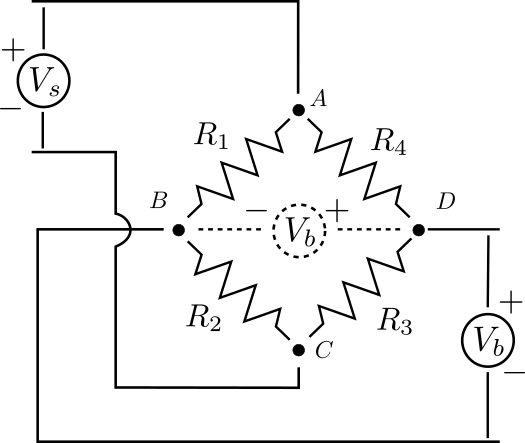
\includegraphics[scale=.35]{bridge_circuit.png} \vspace{15mm} \\ 

Use KVL and the voltage divider rule find the relationship between the two voltages. \vspc
}

% Section III - Frame II:
\frame{
\frametitle{\sectiontitleIII}

}

%% Section IV:
\section{\sectiontitleIV}

% Section IV - Frame I:
\frame{
\frametitle{\sectiontitleIV}
\small

Switches can be used to add a simple user interface to a circuit. There many different types of switches for different purposes. This is not an exhaustive list.

}
	
% Section IV - Frame II:
\frame{
\frametitle{\sectiontitleIV}
\small

Here are a few examples.\vspace{5mm}\\

}


\end{document}





